\newpage
\section{Aufgabe 1: c}

\subsection{Aufgabenstellung}
Für die folgende Aufgabe recherchieren Sie im Internet: Richten Sie die VMs so ein, dass sich die virtuellen Maschinen über das Netzwerk erreichen können (sogenanntes ”Host only”
Netz). Wie erreichen Sie es, dass die virtuellen Maschinen trotzdem Internetzugriff erhalten?
(2 Punkte)

\subsection{Vorbereitung}
Für die Anfertigung dieser Aufgabe benötigen Sie eine Virtualisierungsumgebung(\textit{Oracle VirtualBox}) und zwei, mit \textit{Ubuntu 12.04}, eingerichtete virtuelle Maschinen, nach der Anleitung von \textit{Aufgabe 2} beschrieben.

\subsection{Durchführung}
\begin{enumerate}
	\item Im VirtualBox Manager auf klicken Sie auf \textit{Globale Tools}
	\item Dort wählen Sie \textit{Host-only Netzwerke} aus
		\begin{figure}[H]
			\centering
			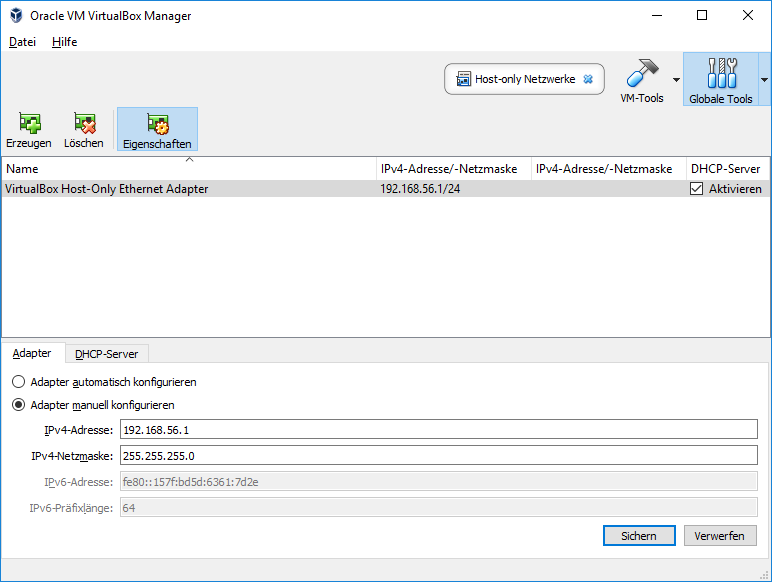
\includegraphics[width=0.4 \linewidth]{images/6}
			\caption{Host-only Netzwerke}
		\end{figure}
		\item Die IP-Konfiguration bleibt auf der voreingestellten Konfiguration, jedoch wird DHCP ausgeschaltet um statische IP-Adressen vergeben zu können
		\begin{figure}[H]
			\centering
			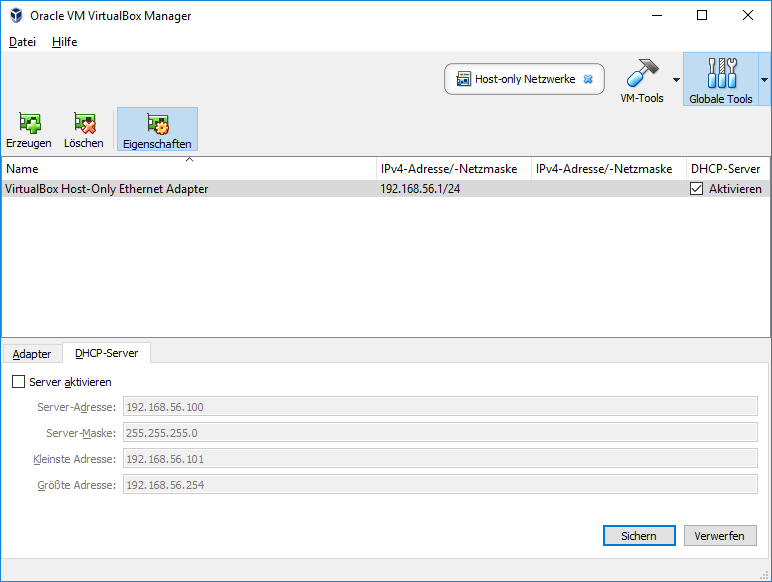
\includegraphics[width=0.4 \linewidth]{images/7}
			\caption{DHCP Konfiguration}
		\end{figure}
		\item Beide virtuelle Maschinen werden im ersten Netzwerkadapter auf Host-Only umgestellt und den eben eingerichteten Host-only Adapter auswählen \\
		\textit{Rechtsklick $\longrightarrow$ Ändern $\longrightarrow$ Netzwerk $\longrightarrow$ Angeschlossen an: Host-only Adapter}
		\begin{figure}[H]
			\centering
			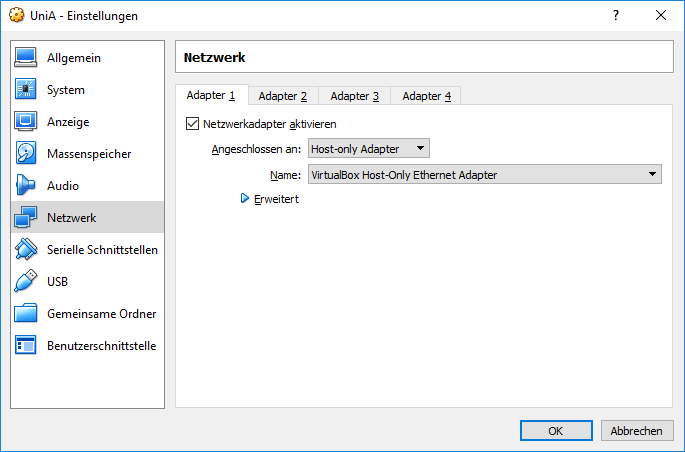
\includegraphics[width=0.4 \linewidth]{images/8}
			\caption{Host-only Einrichtung}
		\end{figure}
		\item Den zweiten Adapter stellen Sie auf NAT um weiterhin den Zugriff auf das Internet gewährleisten zu können
		\begin{figure}[H]
			\centering
			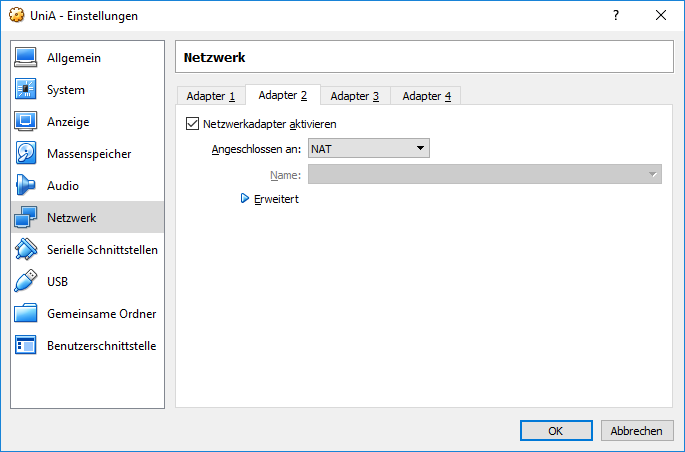
\includegraphics[width=0.4 \linewidth]{images/9}
			\caption{NAT Einrichtung}
		\end{figure}
		\item Starten Sie nun die virtuellen Maschinen
		\item Jetzt stellen Sie die IP-Adressen der jeweiligen virtuellen Maschinen ein \\
		\textit{Systemeinstellung $\longrightarrow$ Netzwerk}\\
		Dort wählen Sie nun Ihre Verbindung aus und klicken auf \textit{Optionen}  \\		\textit{IPv4-Einstellungen $\longrightarrow$ Methode $\longrightarrow$ Manuell} \\ Fügen Sie eine neue Adresse hinzu und geben Sie ihr eine Adresse und eine Netzmaske, in unserem Fall: \\
		\begin{table}[H]
			\tablestyle
			\begin{tabular}{lll}
				\toprule
				& IP-Adresse & Netzmaske \tabularnewline
				
				\midrule
				\textbf{studia} & 192.168.56.101 & 255.255.255.0 \tabularnewline
				\textbf{studib} & 192.168.56.102 & 255.255.255.0 \tabularnewline
			
			\end{tabular}
		\end{table}
		
		\begin{figure}[H]
			\centering
			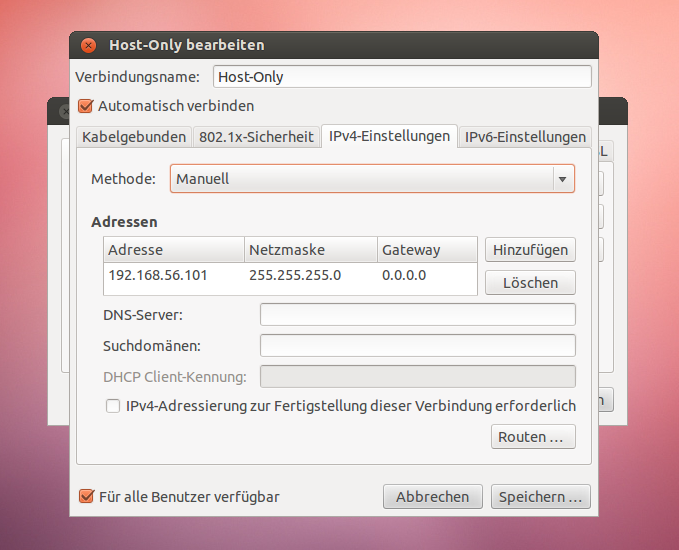
\includegraphics[width=0.4 \linewidth]{images/10}
			\caption{IP-Adressen Einrichtung}
		\end{figure}
\end{enumerate}
Auf Basis von einer Anleitung \cite{long:2013}.

\subsection{Fazit}
Auch diese Aufgabe war einigermaßen leicht zu bearbeiten. Das gesamte Host-Only Netzwerk ist nicht komplexer als gewöhnliche Netzwerkkonfigurationen. Probleme sind während der Bearbeitung nicht aufgetreten. 